\documentclass[acmtocl]{acmtrans2m}
\usepackage{amsmath}
\usepackage{amssymb}
\usepackage{amsfonts}
\usepackage{rotating,tabularx}

\newcommand{\PyTrilinos}{{PyTrilinos}}
\newcommand{\Trilinos}{{Trilinos}}
\newcommand{\TrilinosTM}{Trilinos \copyright}
\newcommand{\trilinos}{{Trilinos}}
\newcommand{\ifpack}{{Ifpack}}
\newcommand{\aztecoo}{{AztecOO}}
\newcommand{\amesos}{{Amesos}}
\newcommand{\epetra}{{Epetra}}
\newcommand{\ml}{{ML}}
\newcommand{\mb}[1]{{\mathbf {#1} }}
\newcommand{\teuchos}{{Teuchos}}
\newcommand{\triutils}{{Triutils}}
\newcommand{\metis}{{METIS}}

\newcommand{\comm}[2]{\bigskip
                      \begin{tabular}{|p{4.5in}|}\hline
                      \multicolumn{1}{|c|}{{\bf Comment by #1}}\\ \hline
                      #2\\ \hline
                      \end{tabular}\\
                      \bigskip
                     }

\acmVolume{0}
\acmNumber{0}
\acmYear{00}
\acmMonth{00}


\newcommand{\BibTeX}{{\rm B\kern-.05em{\sc i\kern-.025em b}\kern-.08em
    T\kern-.1667em\lower.7ex\hbox{E}\kern-.125emX}}

\markboth{M. Sala and W. F. Spotz and M. A. Heroux}{Using Parallel Libraries via
  Python}

\title{PyTrilinos: Using Parallel Distributed Memory Linear Algebra
  Libraries via Python}

\author{Marzio Sala, W. F. Spotz and M. A. Heroux\\Sandia National
  Laboratories}

\begin{abstract}
\PyTrilinos\ is a collection of Python modules that are useful for
serial and parallel scientific computing. This collection contains
modules that cover serial dense linear algebra, parallel sparse linear
algebra, direct and iterative linear solution techniques, domain
decomposition and multilevel preconditioners, nonlinear solvers and
continuation algorithms. Also included are a variety of related
utility functions and classes, including distributed I/O and matrix
generation utilities. \PyTrilinos\ vector objects are integrated with
the popular Numeric Python module, gathering together a variety of
high-level distributed computing operations with serial vector
operations.

PyTrilinos is defined as a set of interfaces to already available
non-Python libraries. This hybrid framework uses Python as front-end,
and efficient pre-compiled libraries for all computationally expensive
tasks. Thus, we take advantage of both the flexibility and ease of use
of Python, and the efficiency of the underlying C++, C and FORTRAN
numerical kernels. The presented numerical results show that, if
properly used, the overhead required by the Python interpreter is
negligible.

To run in parallel, \PyTrilinos\ simply requires a standard Python
interpreter.  The fundamental MPI calls are abstracted beneath the
Epetra module layer, and all inter-processor communications by all
\PyTrilinos\ modules are handled using Epetra communicators. This
makes serial and parallel scripts using \PyTrilinos\ virtually
identical.
\end{abstract}

\category{D.1.3}{Programming Techniques}{Parallel Programming}
\category{D.2.2}{Software Engineering}{Design Tools and Techniques--{\sl
 Object-oriented design methods}}
\category{D.2.13}{Software Engineering}{Reusable Software--{\sl Reusable
  libraries}}
\category{G.1.4}{Numerical Analysis}{General--{\sl Iterative methods}}
\category{G.1.3}{Numerical Analysis}{Numerical Linear Algebra--{\sl
  Sparse, structured, and very large systems (direct and iterative methods)}}
\category{G.1.8}{Numerical Analysis}{Numerical Linear Algebra--{\sl
 Multigrid and multilevel methods}}
\category{G.4}{Mathematical Software}{Algorithm design and analysis}

%\terms{Documentation, Languages}

\keywords{Object-oriented programming, script
  languages, direct solvers, multilevel preconditioners, nonlinear solvers.}
\begin{document}

\setcounter{page}{1}

\begin{bottomstuff}
Authors' address:
PO Box 5800 MS 1110, Albuquerque, NM 87185-1110, U.S.A.\newline
ASCI program and the DOE Office of Science MICS program at Sandia
  National Laboratory.  Sandia is a multiprogram laboratory operated by
  Sandia Corporation, a Lockheed Martin Company, for the United States
  Department of Energy's National Nuclear Security Administration under
  contract DE-AC04-94AL85000.
\end{bottomstuff}

\maketitle

%-----------------------------------------------------------------------------
\section{Introduction}
\label{sec:intro}
%-----------------------------------------------------------------------------

The choice of the programming language for the development and usage
of large-scale, high-performance numerical algorithms is often a
thorny issue. Ideally, the programming language is only a tool used to
produce a working library or application. In practice, there are
important differences between the several programming languages made
available to developers---from FORTRAN77 or FORTRAN90, to C and C++,
Java, Python, MATLAB, and several others. One important distinction
can be made between {\sl interpreted} languages and {\sl compiled}
languages. For the former, the list of instructions (called a {\sl
  script}) is translated at run-time by an interpreter, then executed;
for the latter, the code is compiled and an executable is created.  It
is well known that interpreted code is easier to use and debug, since
the interpreter will analyze each instruction as it is executed. This
comes at a computational price, since the interpreter may require many
CPU cycles (independent of problem size) to parse each instruction.

Therefore, interpreted languages are often disregarded by developers
of high-performance applications or are used only in the concept phase
of application development. Almost all high-performance libraries are
written in compiled languages such as C, C++ or FORTRAN. Since these
languages are reasonably well standardized and compilers quite mature
on almost all platforms, developers can obtain highly efficient and
portable codes.  The downside is that a constant attention to
low-level system programming, like memory allocation and deallocation,
is usually required. Because compilation and linking are essential
steps, the development cycle can be slowed down considerably,
sometimes making the development of new algorithms problematic.

As developers of numerical algorithms, our interest is in a
high-level, flexible programming environment, with performance
comparable to that of native C, C++ or FORTRAN code. Flexibility is
fundamental for rapid prototyping, in the sense that the developer
should be able to write a basic code satisfying his or her needs in a
very short time.  However, it is difficult for a single programming
language to be at the same time
easy-to-use, support rapid development, and produce
optimized executables. Indeed, the goals of efficiency and flexibility
are often in conflict with each other. From our point of view, the key
observation to solve this problem is that, for most applications, the
time-critical portion of the code that requires the efficiency of a
compiled language is related to a small set of self-contained
functions or classes. Therefore, one can adopt an interpreted (and
possibly interactive) language, without a big performance degradation,
provided there is a robust interface between the interpreted and
compiled programs. Among the available scripting languages, we
decided to adopt Python (see, for instance, \cite{python-book}).
Python is an interpreted, interactive, object-oriented programming
language, which combines remarkable power with very clean syntax (it
is often observed that well-written Python code reads like pseudo
code).  Perhaps most importantly, it can be easily extended by using a
variety of open source tools such as SWIG~\cite{swig} to create
wrappers to modules written in C, C++ or FORTRAN for all performance
critical tasks.

This article describes a collection of numerical linear algebra and
solver libraries, called PyTrilinos, built on top of the Trilinos
project~\cite{Trilinos-home-page,Heroux:2005:OTP}.  It adds
significant power to the interactive Python session by exposing the
user to high-level commands and classes for the creation, handling and
usage of serial and distributed, dense and sparse linear algebra
objects. Using \PyTrilinos, an interactive Python session becomes a
powerful data-processing and system-prototyping environment that can
be used to test, validate, use and extend serial and parallel
numerical algorithms. In our opinion, Python naturally complements
languages like C, C++ and FORTRAN rather than competes with them.
Similarly, PyTrilinos complements Trilinos by offering a rapid
development cycle for some of its capabilities.

%Python is a high-level general purpose programming language. Because
%code is automatically compiled to byte code and executed, Python is
%suitable for use as a scripting language.  In typical Python
%development, a system's frontend and infrastructure may be written in
%Python for ease of development and modification, but the kernel is
%still written in C or C++ for efficiency.  We use Python as a glue
%between different modules, written in high-performance languages;
%each of these modules is an already available library, dynamically
%loaded by Python when required.

\smallskip

This article is organized as follows. Section~\ref{sec:design}
describes the project design, the organization of PyTrilinos and its
division into modules. Comments on the usage of parallel, MPI Python
scripts using PyTrilinos are reported in Section~\ref{sec:serial}.  An
overview of how to use PyTrilinos is given in Section~\ref{sec:using}.
Section~\ref{sec:comparison_python} positions PyTrilinos with respect
to similar Python projects.  Section~\ref{sec:comparison_matlab}
compares PyTrilinos with MATLAB.  A comparison between Trilinos and
PyTrilinos implementations is presented in
Section~\ref{sec:comparison_trilinos}.  Performance considerations are
addressed in Section~\ref{sec:performance} and concluding remarks are
given in Section~\ref{sec:concluding}.

%-----------------------------------------------------------------------------
\section{Project Design}
\label{sec:design}
%-----------------------------------------------------------------------------

%-----------------------------------------------------------------------------
\subsection{Why Python and SWIG}
\label{sec:why}
%-----------------------------------------------------------------------------

Python has emerged as an excellent choice for scientific computing
because of its simple syntax, ease of use, object-oriented support and
elegant multi-dimensional array arithmetic. Its interpreted evaluation
allows it to serve as both the development language and the command
line environment in which to explore data. Python also excels as a
``glue'' language between a large and diverse collection of software
packages -- a common need in the scientific arena.

The Simple Wrapper and Interface Generator (SWIG)~\cite{swig} is a
powerful utility that easily facilitates access to C and C++ code from
Python.  SWIG will automatically generate Python (as well as many
other language) interfaces for existing C and C++ code.  It also
supports multiple inheritance and flexible augmentation of the
generated Python interfaces.  Using these features, we can construct
Python classes that derive from two or more disjoint classes and we
can provide custom methods in the Python interface that were not part
of the original C++ interface.

Python combines remarkable power with very clean syntax. It has
modules, namespaces, classes, exceptions, high-level dynamic data
types, automatic memory management that frees the user from most
hassles of memory allocation, and much more. Python also has some
features that make it possible to write large programs, even though it
lacks most forms of compile-time checking: a program can be
constructed out of modules, each of which defines its own
namespace. Exception handling makes it possible to catch errors where
required without cluttering the code with error checking.

Python's development cycle is dramatically shorter than that of
traditional tools. In Python, there are no compile or link
steps---Python programs simply import modules at runtime and use the
objects they contain. Because of this, Python programs run immediately
after changes are made. Python integration tools make it usable in
hybrid, multi-component applications. As one consequence, systems can
simultaneously utilize the strengths of Python for rapid development,
and of traditional languages such as C for rapid execution.  This
flexibility of development modes is crucial in realistic environments.

\subsection{Other Approaches}

Python and SWIG offer one way to obtain a hybrid environment that
combines an interpreted language for high-level development and
libraries for low-level computation with good performance.  Two other
approaches are:

\begin{itemize}

\item MATLAB: An obvious alternative is
  MATLAB~\cite{Matlab-home-page}.  MATLAB provides an intuitive linear
  algebra interface that uses state-of-the-art libraries to perform
  compute-intensive operations such as matrix multiplication and
  factorizations.  MATLAB is the {\it lingua franca} of numerical
  algorithm developers and is used almost universally for algorithm
  prototyping when problem sizes are small, and can in many cases also
  be a production computing environment. However, MATLAB is often not
  sufficient for high-end application because of its limited parallel
  computing support.  MATLAB does support interaction with other
  languages.  It can be used from an application and can use external
  code.  But these capabilities are also quite limited when compared
  to the capabilities of Python and SWIG.  Trilinos does provide some
  MATLAB interoperability through the Trilinos Epetra Extensions
  package, supporting the insertion and extraction of Epetra matrices
  and vector into and from a MATLAB environment, and the execution of
  MATLAB instructions from a C++ program, but this is no substitute
  for a full-featured interactive environment.

\item SIDL/Babel: The Scientific Interface Definition Language (SIDL)
  supports a kind of generic object-oriented interface specification
  that can then be processed by Babel~\cite{Babel-home-page} to
  generate (i) stubs for wrapping an existing library, written in one
  of many supported languages such as Fortran77, Fortran90, C and C++
  and, (ii) multiple language interfaces so that the wrapped libraries
  can be called from any application, regardless of what language the
  application uses.  SIDL/Babel is integral to the development of
  Common Component Architecture (CCA)~\cite{cca} and is an attractive
  solution for libraries that need to support multiple language
  interfaces.  Presently, for the Trilinos project the majority of
  users who want compiled library support are C and C++ programmers,
  so using native Trilinos interfaces, which are written in C++ and C,
  is straight-forward.  Given this fact, SIDL/Babel is not attractive
  because it requires an additional (SIDL) interface specification
  which must be manually synchronized with the native Trilinos C++
  interfaces.  This is labor-intensive and prone to human error.  By
  comparison, SWIG directly includes or imports C/C++ headers, an
  approach which requires no manual synchronization.

\end{itemize}

%-----------------------------------------------------------------------------
\subsection{Multilevel Organization of PyTrilinos}
\label{sec:multilevel}
%-----------------------------------------------------------------------------

\PyTrilinos\ is designed as a modular multilevel framework, and it
takes advantage of several programming languages at different levels.
The key components are:

\begin{enumerate}

\item {\bf Trilinos}, a set of numerical solver packages in active
  development at Sandia National Laboratories that allows
  high-performance scalable linear algebra operations for large
  systems of equations. Trilinos contains more than half a million
  lines of code, and it can interface to many third-party
  libraries. The source code of the current Trilinos public release
  accounts for about 300,000 code lines, divided in about 67,000 code
  lines for distributed linear algebra objects and utilities, 20,000
  code lines for direct solvers and interfaces to third-party direct
  solvers, 128,000 code lines for multilevel preconditioners, and
  76,000 code lines for other algebraic preconditioners and Krylov
  accelerators.

\item {\bf Numeric}, a well-established Python module to handle
  multi-dimensional arrays including vectors and
  matrices~\cite{numeric}.  A large number of scientific packages and
  tools have been written in or wrapped for Python that utilize
  Numeric for representing fundamental linear algebra objects.  By
  integrating with Numeric, PyTrilinos also integrates with this
  sizeable collection of packages.

\item {\bf SWIG}, the Simplified Wrapper and Interface Generator,
  which is a preprocessor that turns ANSI C/C++ declarations into
  scripting language interfaces, and produces a fully working Python
  extension module; see~\cite{swig}.

\item {\bf Distutils}, a Python module with utilities aimed at the
  portable distribution of both pure Python modules and compiled
  extension modules.  Distutils has been a part of the standard Python
  distribution since Python version 2.2.

\end{enumerate}

A description of the organization of the linear algebra modules of
PyTrilinos, with some of the third-party libraries that can be
accessed, is shown in Figure~\ref{fig:organization}.

\begin{figure}
\begin{center}
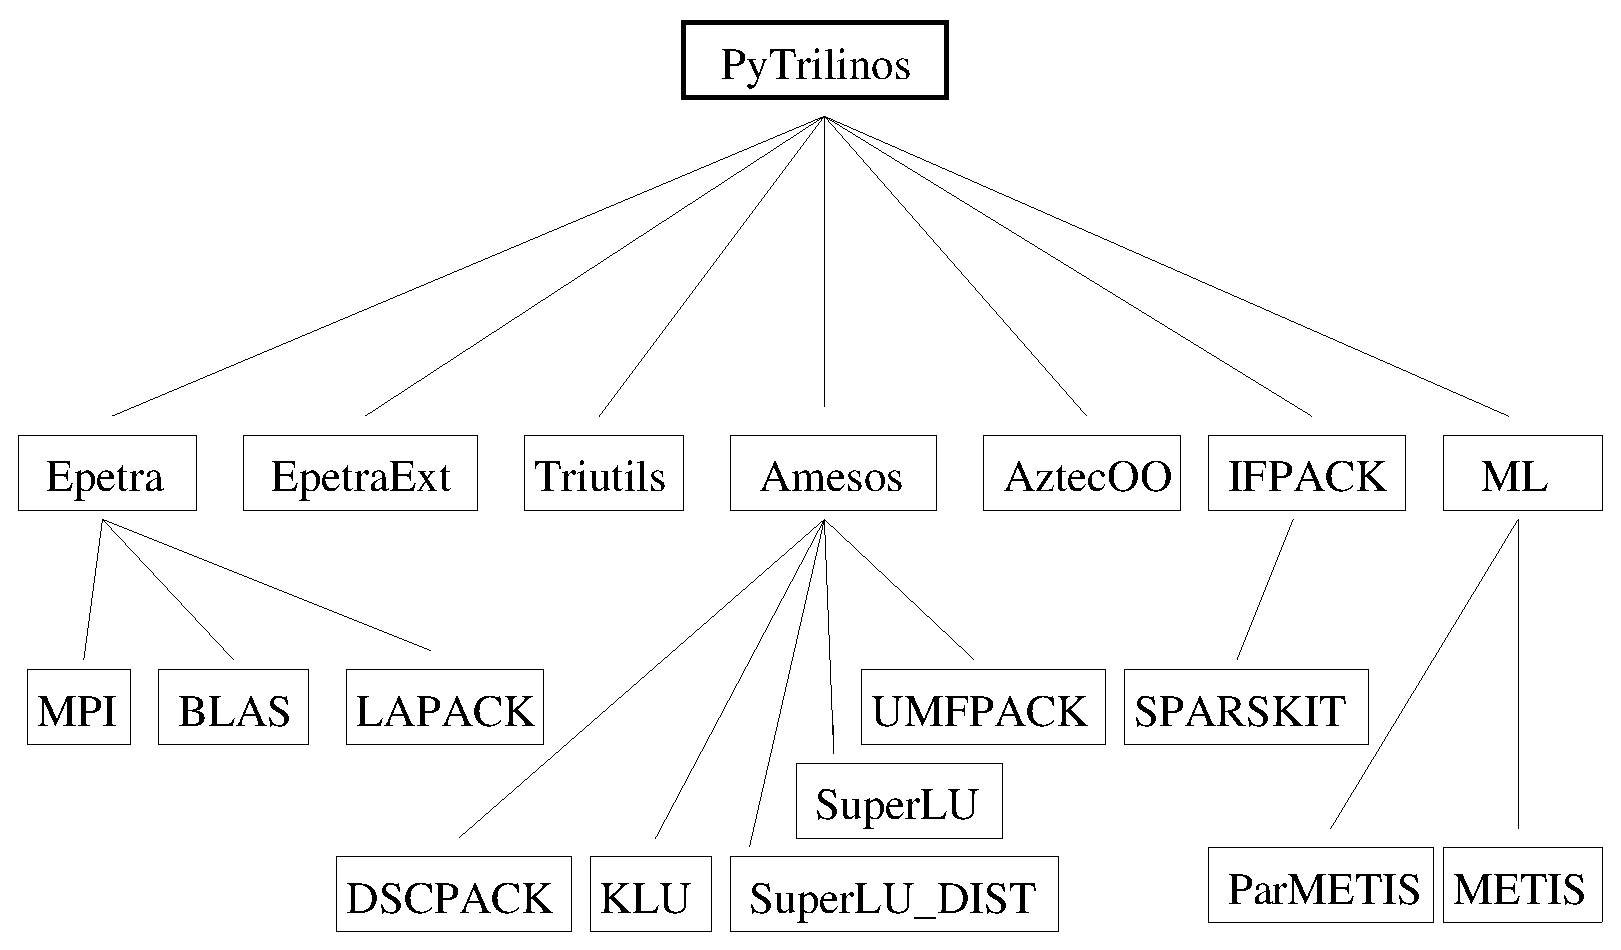
\includegraphics[width=12cm]{organization.eps}
\caption{Organization of the linear algebra modules of PyTrilinos.}
\label{fig:organization}
\end{center}
\end{figure}

%-----------------------------------------------------------------------------
\subsection{PyTrilinos Organization}
\label{sec:organization}
%-----------------------------------------------------------------------------

\PyTrilinos\ reflects the Trilinos organization by presenting a series
of {\sl modules}, each of which wraps a given Trilinos {\sl package},
where a package is an integral unit usually developed by a small team
of experts in a particular area.  Trilinos packages that support
namespaces have a Python submodule for each namespace.  Algorithmic
capabilities are defined within independent packages. At present, the
modules of \PyTrilinos\ are:

\begin{enumerate}

\item {\bf Epetra}, a collection of concrete classes to support the
  construction and use of vectors, sparse distributed graphs, and
  dense and distributed sparse matrices. It provides serial, parallel
  and distributed memory capabilities. Epetra supports
  double-precision floating point data only (no single-precision or
  complex), and uses BLAS and LAPACK where possible, and as a result
  has good performance characteristics.  See~\cite{epetra-guide} for
  more details.

\item {\bf EpetraExt} offers a variety of extension capabilities to
  the Epetra package, such as input/output and coloring algorithms.
  The I/O capabilities make it possible to read and write generic
  Epetra objects (like maps, matrices and vectors).

\item {\bf Triutils} allows the creation of several matrices, like the
  MATLAB's {\tt gallery} function, and it can be useful for examples
  and testing. Some input capabilities make it possible to read a
  matrix in Harwell/Boeing or Matrix Market format, therefore
  accessing a large variety of well-recognized test cases for dense
  and sparse linear algebra.

\item {\bf Amesos} contains a set of clear and consistent interfaces
  to the following third-party serial and parallel sparse direct
  solvers: UMFPACK~\cite{umfpack-acm-toms},
  PARDISO~\cite{oskl:04-etna,sg:04-fgcs},
  TAUCS~\cite{rozin04locality,rotkin04design,irony04parallel}, SuperLU and
  SuperLU\_DIST~\cite{superlu-manual}, DSCPACK~\cite{dscpack-manual},
  MUMPS~\cite{mumps-manual}, and
  ScaLAPACK~\cite{scalapack-book,scalapack}. As such,
  \PyTrilinos\ makes it possible to access state-of-the-art direct
  solver algorithms developed by groups of specialists, and written in
  different languages (C, FORTRAN77, FORTRAN90), in both serial and
  parallel environments. By using Amesos, more than 350,000 code lines
  (without considering BLAS, LAPACK, and ScaLAPACK) can be easily
  accessed from any code based on Trilinos (and therefore PyTrilinos).
  We refer to~\cite{Amesos-Reference-Guide,Amesos-Design}
  for more details.

\item {\bf AztecOO} contains preconditioned Krylov accelerators, like
  CG, GMRES and several others~\cite{golub96matrix}, based on the
  popular Aztec library~\cite{aztecoo-guide}.  One-level domain
  decomposition preconditioners based on incomplete factorizations are
  available.

\item {\bf IFPACK} contains object-oriented algebraic preconditioners,
  compatible with Epetra and AztecOO.  It supports construction and
  use of parallel distributed memory preconditioners such as
  overlapping Schwarz domain decomposition with several local solvers.
  IFPACK can take advantage of SPARSKIT~\cite{sparskit}, a widely used
  software package; see~\cite{ifpack-guide}.

\item {\bf ML} contains a set of multilevel preconditioners based on
  aggregation procedures for serial and vector problems compatible
  with Epetra and AztecOO. ML can take advantage of the
  METIS~\cite{metis} and ParMETIS~\cite{parmetis} libraries to create
  the aggregates.  For a general introduction to ML and its
  applications, we refer to the ML Users Guide~\cite{ml-guide}.

\item {\bf NOX} is a collection of nonlinear solver algorithms.  NOX
  is written at a high level with low level details such as data
  storage and residual computations left to the user.  This is
  facilitated by interface base classes which users can inherit from
  and define concrete methods for residual fills, Jacobian matrix
  computation, etc.  NOX also provides some concrete classes which
  interface to Epetra, LAPACK, PETSc and others.  For Python, a
  PyInterface class has been defined, designed to work with
  Epetra.Vectors.

\end{enumerate}

Note that all third-party libraries (except BLAS and LAPACK) are
optional and do not need to be installed to use \PyTrilinos\ (or
Trilinos).

All the presented modules depend on Epetra, since Epetra is the
``language'' of Trilinos, and offers a convenient set of interfaces to
define distributed linear algebra objects.  \PyTrilinos\ cannot be
used without the Epetra module, while all the other modules can be
enabled or disabled in the configuration phase of Trilinos.

Epetra.Vector objects have been designed to multiply inherit, not only
from the Epetra\_Vector C++ class, but the Numeric UserArray Python
class.  The constructors are written to ensure that the internal data
pointers of both classes point to the same buffer in memory so that
the Python programmer can treat an Epetra.Vector either type of linear
algebra object.

%-----------------------------------------------------------------------------
\section{Serial and Parallel Environments}
\label{sec:serial}
%-----------------------------------------------------------------------------

Although testing and development of high-performance algorithms can be
done in serial environments, parallel environments still constitute
the most important field of application for most of Trilinos'
algorithms. However, Python itself does not provide any parallel
support. Because of this, several projects have been developed
independently, to fill the gap between Python and MPI applications. We
have analyzed the following:

\begin{itemize}

\item {\bf MPI Python (pyMPI)} is a framework for developing parallel
  Python applications using MPI~\cite{MPI-Python};

\item {\bf PyPAR} is a more light-weight wrapper of the MPI library
  for Python~\cite{pypar}.

\item {\bf Python BSP} supports the more high-level Bulk Synchronous
  Parallel approach~\cite{bsp}

\end{itemize}

All of these projects allow the use of Python through the interactive
prompt, but additional overhead is introduced. Also, none of these
projects define a well-recognized standard, since they are still
under active development.

Our approach is somewhat complementary to the efforts of these
projects.  We decided to use a standard, out-of-the-box, Python
interpreter, then wrap only the very basic of MPI: MPI\_Init(),
MPI\_Finalize(), and MPI\_COMM\_WORLD. By wrapping these three
objects, one can define an MPI-based Epetra communicator, on which all
wrapped Trilinos packages are already based. This reflects the
philosophy of all the considered Trilinos packages, that have no
explicit dependency on MPI communicators, and accept the pure virtual
class Epetra\_Comm instead. PyTrilinos scripts can create a
specialized communicator using command
\begin{verbatim}
    >>> comm = Epetra.PyComm()
\end{verbatim}
which returns an Epetra.SerialComm if \PyTrilinos\ has been compiled
in serial mode, or an Epetra.MpiComm if \PyTrilinos\ has support for
MPI. By using Epetra.PyComm, \PyTrilinos\ scripts are virtually
identical for both serial and parallel runs, and generally reads:
\begin{verbatim}
    >>> from PyTrilinos import Epetra
    >>> Epetra.Init()
    >>> comm = Epetra.PyComm()
        ...
    >>> Epetra.Finalize()
\end{verbatim}
A pictorial representation of how communication are handled in the
case of two processors is given in Figure~\ref{fig:distributed}. For
serial runs, both Init() and Finalize() are empty instructions; for
parallel runs, Init() calls MPI\_Init() and Finalize() finalizes the
MPI environment.

\smallskip

The major disadvantages of this approach are that Python cannot be run
interactively if more than one processor is used, and we experienced
problems with some MPI interpreters (in particular MPICH) to execute
Python scripts.  Although all the most important MPI calls are
available through Epetra.Comm objects (for example, the rank of a
process is returned by method {\tt Comm.MyPID()} and the number of
processes involved in the computation by method {\tt Comm.NumProc()}),
not all the functions specified by the MPI forum are readily available
through the Comm object.  For example, there are no point-to-point
communications, or non-blocking functions. Also, PyTrilinos always
uses MPI\_COMM\_WORLD as its basic communicator.

In our opinion, these are only minor drawbacks, and the list of
advantages is much longer. First, since all calls are handled by
Epetra, no major overhead occurs, other than that of parsing a Python
instruction. Second, all PyTrilinos modules that require direct MPI
calls can dynamically cast the Epetra.Comm object, retrieve the MPI
communicator object, then use direct C/C++ MPI calls. As such, the
entire set of MPI function is available to developers with no
additional overhead. Third, a standard Python interpreter is
used. Finally, serial and parallel scripts can be identical, and
PyTrilinos scripts can be run in parallel by using an instruction of
type
\begin{verbatim}
    % mpirun -np 4 python my-script.py
\end{verbatim}
at the shell prompt, where {\tt my-script.py} contains at least the basic
instructions required to define an Epetra.PyComm.

One should note that, in addition to Epetra.PyComm which is defined
differently depending on whether MPI support is enabled,
Epetra.SerialComm and Epetra.MpiComm will always produce serial and
MPI implementations of the Epetra.Comm base class, respectively.
Thus, nesting of serial communicators within an MPI application is
possible.

\begin{figure}
\begin{center}
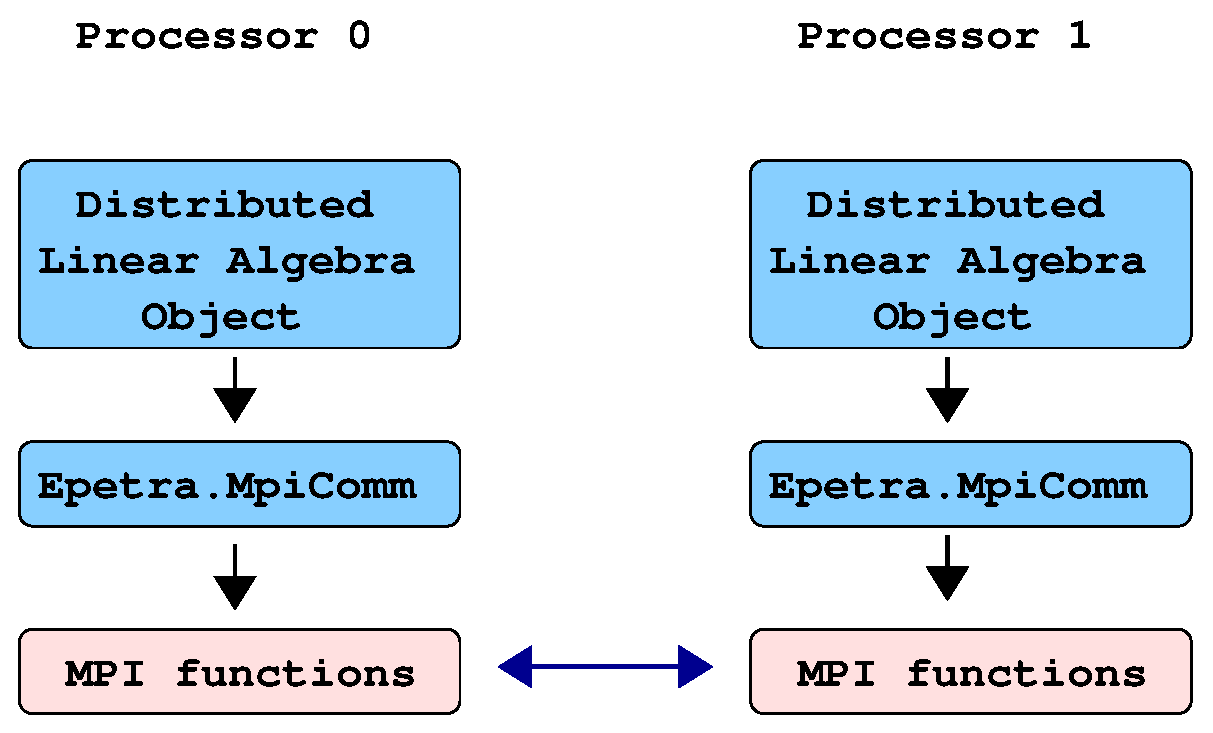
\includegraphics[height=5cm]{distributed_object.eps}
\caption{All distributed PyTrilinos objects are constructed with the
  Epetra.MpiComm object, which takes care of calling MPI functions for
  inter-processor communications.}
\label{fig:distributed}
\end{center}
\end{figure}


%-----------------------------------------------------------------------------
\section{Using PyTrilinos}
\label{sec:using}
%-----------------------------------------------------------------------------

In order to present the functionalities of PyTrilinos, this section
will briefly describe the main capabilities of all modules, together
with a brief mathematical background of the implemented algorithms.
More technical details on the usage of the linear algebra modules of
PyTrilinos can be found in~\cite{pytrilinos-la-guide}.

%-----------------------------------------------------------------------------
\subsection{The Epetra Module}
\label{subsec:epetra}
%-----------------------------------------------------------------------------

The Epetra module offers a large variety of objects for linear algebra
and parallel processing. The most basic objects are the {\sl
  communicator}, which encapsulates all the inter-processor data
exchange, and the {\sl map}, which describes the domain decomposition
of distributed linear algebra objects. Serial runs make use of trivial
communicators and maps; parallel runs adopt an MPI-based communicator
and support arbitrary maps.

Several other functionalities are offered by Epetra:

\begin{itemize}

\item Epetra provides an extensive set of classes to create and fill
  distributed sparse matrices. These classes allow row-by-row or
  element-by-element constructions. Support is provided for common
  matrix operations, including scaling, norm, matrix-vector
  multiplication and matrix-multivector multiplication.  Compressed
  row sparse matrices can be stored row-by-row using class
  Epetra.CrsMatrix. This class is derived from the pure abstract class
  Epetra.RowMatrix, and as such it can be used with all the linear
  algebra modules of PyTrilinos.

\item Non-local matrix elements can be set using class
  Epetra.FECrsMatrix.

\item Distributed vectors (whose local component is at the same time a
  Numeric vector) can be handled with classes Epetra.Vector and
  Epetra.MultiVector. Operations like norms and AXPY's are supported.

\item Distributed graphs can be created using class Epetra.CrsGraph.

\item Serial dense linear algebra is supported (as a light-weight
  layer on the top of BLAS and LAPACK) through classes
  Epetra.SerialDenseVector and Epetra.SerialDenseMatrix.

\item Several utilities are available, for example Epetra.Time offers
  a clean an consistent access to timing routines.

\end{itemize}

%-----------------------------------------------------------------------------
\subsection{The Triutils Module}
\label{subsec:triutils}
%-----------------------------------------------------------------------------

The Triutils module provides:

\begin{itemize}

\item Matrix reading capabilities: A function is available to read a
  matrix from the popular Harwell/Boeing format.

\item Matrix generation capabilities. Several matrices, corresponding
  to finite difference discretization of model problems, can be
  generated using the matrix gallery of Triutils, which provides
  functionalities similar to that of the MATLAB's {\tt gallery}
  command; see~\cite[Chapter 5]{Trilinos-tutorial} for more details.

\end{itemize}

This module is intended mainly for testing linear solvers.

%-----------------------------------------------------------------------------
\subsection{The Amesos Module}
\label{subsec:amesos}
%-----------------------------------------------------------------------------

Once a (square) sparse matrix and two vectors or multivectors are
created, an important problem is how to solve the corresponding linear
system
\begin{equation}
  \label{eq:lin_sys}
  A X = B
\end{equation}
where $A \in \mathbb{R}^{n \times n}$ is a sparse linear operator, $X
\in \mathbb{R}^{n \times m}$ and $B \in \mathbb{R}^{n \times m}$ are
the solution and right-hand sides, respectively. Parameter $n$ is the
global dimension of the problem, and $m$ is the number of vectors in
the multi-vectors $X$ and $B$.  (If $m = 1$, then $X$ and $B$ are
``standard'' vectors.)  Linear systems of type (\ref{eq:lin_sys})
arise in a variety of applications, and constitute the innermost
computational kernel, and often the most time-consuming of several
numerical algorithms. An efficient solver for Equation
(\ref{eq:lin_sys}) is of fundamental importance for most PDE solvers,
both linear and non-linear.

\smallskip

Typically, the most robust strategy to solve (\ref{eq:lin_sys}) is to
factor the matrix $A$ into the product of two matrices $L$ and $U$, so
that $A = L \, U$, and the linear systems with $L$ and $U$ are readily
solvable. Usually, $L$ and $U$ are a lower and upper triangular
matrix, respectively, and the process is referred to as LU
decomposition. In PyTrilinos, the direct solution of large linear
systems is performed by the Amesos module, which defines interfaces to
third-party direct solvers. All Amesos objects are constructed from
the function class {\tt Amesos}.  The main goal of this class is to
allow the user to select any supported direct solver (that has been
enabled at configuration time) by simply changing an input
parameter. An example of a script reading the linear system stored in
the Harwell/Boeing format, then solving the problem using SuperLU is
shown in Figure~\ref{fig:amesos}.  Several parameters, specified using
Python's dictionaries, are available to toggle the selected Amesos
solver. These parameters share the same name used by Trilinos codes; a
list of available parameters can be found in the Amesos
manual~\cite{Amesos-Reference-Guide}. Note that, just by changing the
value of \verb!SolverType!, the {\sl same} script can be used to
experiment with all the solvers supported by Amesos.

\begin{figure}
  \begin{center}
    \begin{tabular}{| p{12cm} |}
      \hline \\
      \footnotesize
      \begin{minipage}{11.5cm}
\begin{verbatim}
from PyTrilinos import Amesos, Triutils, Epetra

Epetra.Init()
Comm = Epetra.PyComm()
Map, Matrix, LHS, RHS, Exact = Triutils.ReadHB("fidap035.rua", Comm)

Problem = Epetra.LinearProblem(Matrix, LHS, RHS);
Factory = Amesos.Factory()
SolverType = "SuperLU"
Solver = Factory.Create(SolverType, Problem)
AmesosList = {"PrintTiming" : True,
              "PrintStatus" : True  }
Solver.SetParameters(AmesosList)
Solver.SymbolicFactorization()
Solver.NumericFactorization()
Solver.Solve()
LHS.Update(-1.0, Exact, 1.0)
ierr, norm = LHS.Norm2()
print '||x_computed - x_exact||_2 = ', norm
Epetra.Finalize()
\end{verbatim}
      \end{minipage}
      \\
      \\
      \hline
    \end{tabular}
    \caption{Complete script that solves a linear system using
      Amesos/SuperLU.}
    \label{fig:amesos}
  \end{center}
\end{figure}

%-----------------------------------------------------------------------------
\subsection{The AztecOO, IFPACK and ML Modules}
\label{subsec:aztecoo_ifpack}
%-----------------------------------------------------------------------------

For a sparse matrix, the major inconvenience of direct solution
methods (as presented in section \ref{subsec:amesos}) is that the $L$
and $U$ factors are typically much denser than the original matrix
$A$, making LU decomposition too memory demanding for large scale
problems. Moreover, the factorization process is inherently serial,
and parallel factorization algorithms can be successfully used only
with a relatively modest number of processors. The forward and back
triangular solves typically exhibit very poor parallel speedup.

A very well known solution to this problem is to adopt an iterative
solution process, like conjugate gradient or
GMRES~\cite{golub96matrix}. The rationale behind iterative methods
is that they only require (at least in their simplest form)
matrix-vector and vector-vector operations, and both classes of
operations scale well.

Unfortunately, the convergence of iterative methods is determined by
the spectral properties of the matrix $A$---typically, its condition
number $\kappa(A)$.  For real-life problems $\kappa(A)$ is often
``large'', meaning that the iterative solution method will converge
slowly. To solve this problem, the original linear system is replaced
by
\[
A P^{-1} P X = B
\]
where $P$, called a {\sl preconditioner}, is an operator whose inverse
aims to represent the inverse of $A$, though being much cheaper to
compute.  $P$ is chosen so that $AP^{-1}$ is easier to solver than $A$
(that is, it is better conditioned), both in terms of iterations to
converge and CPU time.

\smallskip

Often, algebraic preconditioners are adopted, that is, $P$ is
constructed by manipulating the entries of $A$. This gives rise to the
so-called incomplete factorization preconditioners (ILU) or algebraic
multilevel methods.

Because ILU preconditioners do not scale well on parallel computers, a
common practice is to perform {\em local} ILU factorizations.  In this
situation, each processor computes a factorization of a subset of
matrix rows and columns independently from all other processors.
What we have just described is an example of one-level overlapping
domain decomposition (DD) preconditioners.  The basic idea of DD
methods consists in dividing the computational domain into a set of
subdomains, which may or may not overlap. We will focus on overlapping
DD methods only, because they can be re-interpreted as algebraic
manipulation of the assembled matrix, thus allowing the construction
of black-box preconditioners. Overlapping DD methods are often
referred to as overlapping Schwarz methods. DD preconditioners can be
written as
\begin{equation}
  \label{eq:prec_dd}
  P^{-1} = \sum_{i=1}^M R_i^T B_i^{-1} R_i,
\end{equation}
where $M$ represents the number of subdomains, $R_i$ is a rectangular
Boolean matrix that restricts a global vector to the subspace defined
by the interior of the $i$th subdomain, and $B_i^{-1}$ approximates
the inverse of
\begin{equation}
  \label{eq:aztecoo_tilde_a}
  A_i = R_i A R_i^T,
\end{equation}
for example, being its ILU factorization.

\medskip

To adopt an iterative solver (for example, CG), with 1550 maximum
iterations and a tolerance of $10^{-5}$ on the relative residual,
\PyTrilinos\ requires the instructions shown in
Figure~\ref{fig:aztecoo}. The script creates a preconditioner defined by
(\ref{eq:prec_dd}), using AztecOO's factorizations to solve the local
problems. The sparsity pattern of a matrix is visualized with the
instruction \verb!PrintSparsity()! of the IFPACK module; an example of
output is shown in Figure~\ref{fig:sparsity}. IFPACK can also be used
to define other flavors of domain decomposition preconditioners.

\begin{figure}
  \begin{center}
    \includegraphics[height=5cm]{sparsity.ps}
    \caption{Plot of sparsity pattern of a matrix obtained using
      {\tt IFPACK.PrintSparsity()}.}
    \label{fig:sparsity}
  \end{center}
\end{figure}

\begin{figure}
  \begin{center}
    \begin{tabular}{| p{12cm} |}
      \hline
      \\
      \footnotesize
      \begin{minipage}{11.5cm}
\begin{verbatim}
from PyTrilinos import IFPACK, AztecOO, Triutils, Epetra

Epetra.Init()
Comm = Epetra.PyComm()
Map, Matrix, LHS, RHS, Exact = Triutils.ReadHB("fidap035.rua", Comm)

IFPACK.PrintSparsity(Matrix, "matrix.ps")

Solver = AztecOO.AztecOO(Matrix, LHS, RHS)
Solver.SetAztecOption(AztecOO.AZ_solver, AztecOO.AZ_cg)
Solver.SetAztecOption(AztecOO.AZ_precond, AztecOO.AZ_dom_decomp)
Solver.SetAztecOption(AztecOO.AZ_subdomain_solve, AztecOO.AZ_ilu)
Solver.SetAztecOption(AztecOO.AZ_graph_fill, 1)
Solver.Iterate(1550, 1e-5)
Epetra.Finalize()
\end{verbatim}
      \end{minipage}
      \\
      \\
      \hline
    \end{tabular}
    \caption{Complete example of usage of AztecOO.}
    \label{fig:aztecoo}
  \end{center}
\end{figure}

\medskip

Another class of preconditioner is given by multilevel
preconditioners.  For certain combinations of iterative methods and
linear systems, the error at each iteration projected onto the
eigenfunctions has components that decay at a rate proportional to the
corresponding eigenvalue (or frequency).  Multilevel methods exploit
this property \cite{Briggs} by projecting the linear system onto a
hierarchy of increasingly coarsened ``meshes'' so that each error
component rapidly decays on at least one coarse ``mesh.''  The linear
system on the coarsest ``mesh,'' called the coarse grid problem, is
solved directly.  The iterative method is called the smoother, as a
reflection of its diminished role as a way to damp out the high
frequency error.  The grid transfer (or interpolation) operators are
called restriction and prolongation operators.

Multilevel methods are characterized by the sequence of coarse spaces,
the definition of the operators for each coarse space, the
specification of the smoother, and the restriction and prolongation
operators.  Geometric multigrid (GMG) methods are multilevel methods
that require the user to specify the underlying grid, and in most
cases a hierarchy of (not necessarily nested) coarsened grids.

Algebraic multigrid (AMG) (see \cite[Section 8]{Briggs}) method
development has been motivated by the demand for multilevel methods
that are easier to use.  In AMG, both the matrix hierarchy and the
prolongation operators are constructed just from the stiffness matrix.
To use Aztec00 or IFPACK, a user must supply a linear system and
select a preconditioning strategy.  In AMG, the only additional
information required from the user is to specify a coarsening
strategy.

Using the ML module, the user can easily create black-box two-level
and multilevel preconditioners based on smoothed aggregation
procedures (see \cite{sala04analysis,brezina97robust} and the
references therein). Parameters are specified using a Python
dictionary, as presented for the Amesos module in
Section~\ref{subsec:amesos}; the list of accepted parameters is given
in~\cite{ml-guide}. Applications using ML preconditioners have been
proved to be scalable up to thousands of
processors~\cite{ijnme,shadid-jcp-dd-precond}.

%-----------------------------------------------------------------------------
\subsection{The EpetraExt Module}
\label{subsec:epetraext}
%-----------------------------------------------------------------------------

The EpetraExt module offers a variety of extension to the Epetra
module, such as matrix-matrix operations (addition, multiplication and
transformation), graph coloring algorithms and reading and writing
capabilities of important Epetra objects. For example, to read a
vector and a matrix stored in Matrix-Market format, one simply has to
write:
\begin{verbatim}
    >>> (ierr, X2) = EpetraExt.MatrixMarketFileToMultiVector("x.mm", Map)
    >>> (ierr, A2) = EpetraExt.MatrixMarketFileToCrsMatrix("A.mm", Map)
\end{verbatim}
EpetraExt defines a powerful tool for exchanging data between C++
codes written with Trilinos and Python codes written with
\PyTrilinos. Users can load up distributed Trilinos objects, obtained
with production codes and stored in a file using the EpetraExt
package, then use Python to validate the code, or perform fine-tuning
of numerical algorithms.

%-----------------------------------------------------------------------------
\subsection{The NOX Module}
\label{subsec:nox}
%-----------------------------------------------------------------------------

The NOX module is intended to solve nonlinear problems of the form
\begin{equation}
  \label{eq:nonlinear}
  F(x^*) = 0,
\end{equation}
where $F$ is a nonlinear system of equations defined for a vector of
unknowns $x$, whose (possibly non-unique) solution is given by
$x=x^*$.  NOX supports a variety of algorithms for
solving~(\ref{eq:nonlinear}), all of which utilize a common interface
framework for passing data and parameters between the user's top-level
code and underlying NOX routines.

This framework takes the form of a base class that we inherit from and
that supports a given data format, for example {\tt
  NOX::Epetra::Interface} {\tt NOX::LAPACK::Interface} or {\tt
  NOX::Petsc::Interface}.  Our derived class then implements the
method {\tt computeF} with arguments for input $x$ and the result $F$.
Depending on the algorithm employed, other methods may be required,
and include {\tt computeJacobian}, {\tt computePrecMatrix} and {\tt
  computePreconditioner}.

The Python implementation of NOX supports the Epetra interface.
However, additional code was required to ensure NOX could call back to
python and that the data would be passed between NOX and Python
correctly.  To achieve this, an new interface named {\tt PyInterface}
was developed:
\begin{verbatim}
    from PyTrilinos import NOX
    class Problem(NOX.Epetra.PyInterface):
        def computeF(self, x, rhs):
            ...
            return True
\end{verbatim}
When NOX needs the function $F$ to be computed, it will send {\tt x}
and {\tt rhs}, via the {\tt PyInterface} class, to {\tt computeF} as
{\tt Epetra.Vector}s.  The method should {\tt return} a Boolean
indicating whether the computation was successful or not.  If
required, the methods {\tt computeJacobian}, {\tt computePrecMatrix}
and {\tt computePreconditioner} may also be provided.

Typically, our derived class can become quite extensive, with a
constructor and set and get methods for physical parameters, mesh
information and meta-information such as graph connectivity.  But
minimally, all that is required is a {\tt computeF} method.  We will,
however, have to provide an {\tt Epetra\_Operator} that computes the
Jacobian for our system.  NOX provides a way to approximate the
Jacobian using a finite difference formula:
\begin{equation}
  J_{ij} = \frac{\partial F_i}{\partial x_j} = \frac{F_i(x+\delta e_j)
    - F_i(x)}{\delta}
\end{equation}
where $J=\{J_{ij}\}$ is the Jacobian matrix, $\delta$ is a small
perturbation, and $e_j$ is the cartesian unit vector for dimension
$j$.  This operator can be constructed as follows:
\begin{verbatim}
    from PyTrilinos import Epetra
    comm    = Epetra.SerialComm()
    map     = Epetra.Map(n,0,comm)
    iGuess  = Epetra.Vector(map)
    problem = Problem()
    jacOp   = NOX.Epetra.FiniteDifference(problem, iGuess)
\end{verbatim}
This operator is then passed to the {\tt Group} constructor, which
defines the nonlinear system:
\begin{verbatim}
    group = NOX.Epetra.Group(prParams, lsParams, problem, iGuess, jacOp)
\end{verbatim}
where {\tt prParams} and {\tt lsParams} are {\tt NOX.Parameter.List}s
with printing and linear system parameters, respectively.  They are
typically set via
\begin{verbatim}
    nlParams = NOX.Parameter.List()
    nlParams.setParameter("Nonlinear Solver", "Line Search Based")
    prParams  = nlParams.sublist("Printing")
    prParams.setParameter("Output Precision", 3)
    ...
    dirParams = nlParams.sublist("Direction")
    dirParams.setParameter("Method", "Newton")
    newtonParams = dirParams.sublist("Newton")
    newtonParams.setParameter("Forcing Term Method", "Constant")
    lsParams = newtonParams.sublist("Linear Solver")
    lsParams.setParameter("Aztec Solver", "GMRES")
    ...
\end{verbatim}
See the NOX documentation for details on building parameter lists.  We
are almost ready to construct a solver manager.  All we need is our
group, the top-level parameter list, and a stopping criterion:
\begin{verbatim}
    relResid = NOX.StatusTest.NormF(group, 1.0e-6)
    solver   = NOX.Solver.Manager(group, relResid, nlParams)
\end{verbatim}
All of the NOX {\tt StatusTest} classes are supported, including {\tt
  Combo}, for building compund stopping tests.  Now all that is left
to do is execute the solver and extract the results.
\begin{verbatim}
    status = solver.solve()
    print "\nStatus test:"
    if (status == NOX.StatusTest.Converged):
        print "Nonlinear solver converged!"
        nlOutParams = nlParams.sublist("Output")
        lsOutParams = lsParams.sublist("Output")
        nlIts = nlOutParams.getParameter("Nonlinear Iterations")
        lsIts = lsOutParams.getParameter("Total Number of Linear Iterations")
        resid = nlOutParams.getParameter("2-Norm of Residual")
        print "Nonlinear its = %d, total linear its = %d, residual = %f" \
              % (nlIts, lsIts, resid)
\end{verbatim}
We note that the {\tt FiniteDifferencing} operator is extremely
inefficient and that the computation of Jacobians for sparse systems
can be sped up considerably by using the {\tt
  NOX.Epetra.FiniteDifferenceColoring} operator instead, along with
the graph coloring algorithms in {\tt EpetraExt}.

%-----------------------------------------------------------------------------
\section{Comparison Between PyTrilinos and Related Python Projects}
\label{sec:comparison_python}
%-----------------------------------------------------------------------------

This Section positions PyTrilinos with respect to the following related
Python projects:

\begin{itemize}

\item {\bf Numeric.} The Python Numeric module adds a fast, compact,
  multidimensional array language facility to Python.  Many existing
  scientific software packages for Python (plotting packages, for
  example) accept or expect Numeric arrays as arguments.  To increase
  the compatibility of \PyTrilinos\ with this large collection of
  packages, the fundamental \PyTrilinos\ vector class, {\tt
    Epetra.Vector}, inherits from both the C++ {\tt Epetra\_Vector}
  and the Python Numeric {\tt UserArray} classes.  Thus a {\tt
    Epetra.Vector} {\sl is} a Numeric array, and can be treated as
  such with other Python modules.  However, note that a Numeric array
  is {\sl not} recognized as a {\tt Epetra\_Vector}, since all
  distributed Epetra objects requires an underlying communicator and
  map (not supported by Numeric).

  {\bf Some of this has already been discussed in Section 2.4...}

\item {\bf NumArray.}  NumArray is a reimplementation of Numeric which
  adds the ability to efficiently manipulate large contiguous-data
  arrays in ways similar to MATLAB.  Many scientific Python packages
  have begun the migration from Numeric to NumArray; \PyTrilinos\
  developers are currently exploring the possibility.

  {\bf Why aren't we using NumArray?}

\item {\bf SciPy.} SciPy is an open source library of scientific tools
  for Python. SciPy supplements the popular Numeric module, gathering
  a variety of high level science and engineering modules together as
  a single package. SciPy includes modules for graphics and plotting,
  optimization, integration, special functions, signal and image
  processing, genetic algorithms, ODE solvers, and others.

  {\bf Why aren't we using SciPy?}

\item {\bf ScientificPython.}  ScientificPython is a collection of
  Python modules that are useful for scientific computing. In this
  collection you will find modules that cover basic geometry (vectors,
  tensors, transformations, vector and tensor fields), Quaternions,
  automatic derivatives, (linear) interpolation, polynomials,
  elementary statistics, nonlinear least-square fits, unit
  calculations, Fortran-compatible text formatting, 3D visualization
  via VRML, and Tk widgets for simple line plots and 3D wireframe
  models. There are also interfaces to the netCDF library (portable
  structured binary files), to MPI (Message Passing Interface), and to
  BSPlib (Bulk Synchronous Parallel programming).

  {\bf Why aren't we using ScientificPython?}

\item {\bf PySparse.}  PySparse~\cite{broker05using} can handle
  symmetric and non-symmetric serial sparse matrices, and contains a
  set of iterative methods for solving linear systems of equations,
  preconditioners, an interface to a serial direct solver (SuperLU),
  and an eigenvalue solver for the symmetric, generalized matrix
  eigenvalue problem.  PySparse is probably the first successful
  public-domain software that offers efficient sparse matrix
  capabilities in Python. However, in our opinion PyTrilinos allows
  the user to access a much larger set of well-tested algorithms
  (including nonlinear solvers) in a more modular way.  Also,
  PySparse cannot be used in a parallel environments while PyTrilinos
  can.

\end{itemize}

%-----------------------------------------------------------------------------
\section{Comparison Between PyTrilinos and MATLAB}
\label{sec:comparison_matlab}
%-----------------------------------------------------------------------------

Any mathematical software framework which claims ease-of-use cannot
avoid a comparison with MATLAB, the {\sl de-facto} standard for the
development of numerical analysis algorithms and software.
Our
experience is that, while MATLAB's vector syntax and built-in matrix
data types greatly simplifies the programming language, it is not
possible to perform large-scale computing using this language.
MATLAB's sparse matrix operations are slow compared with Epetra's, as later
shown in this Section.
Another handicap of MATLAB is the inflexibility of its scripting
language: There may be only one visible function in a file, and the
function name must be the file name itself. This can make it harder to
modularize the code. Other desirable language features, such as
exception handling, are also missing in MATLAB.

We now present some numerical results that compare the CPU time required by
PyTrilinos and MATLAB 7.0 (R14) to create a dense and a sparse matrix.
The first test sets the elements of a serial dense matrix, where each
$(i,j)$ element of the square real matrix $A$ is defined as $A(i,j) =
1/(i + j)$. The corresponding MATLAB code reads as follows:
\begin{verbatim}
    A = zeros(n, n);
    for i=1:n
      for j=1:n
        A(i,j) = 1.0/(i + j);
      end
    end
\end{verbatim}
while the PyTrilinos code is:
\begin{verbatim}
    A = Epetra.SerialDenseMatrix(n, n)
    for i in xrange(4):
      for j in xrange(4):
        A[i,j] = 1.0 / (i + j + 2)
\end{verbatim}
From Table~\ref{tab:matlab_dense}, it is evident that MATLAB is more
efficient than PyTrilinos in the handling of dense matrices.

The second test creates a sparse diagonal matrix, setting
one element at a time. The MATLAB code reads:
\begin{verbatim}
    A = spalloc(n, n, n);
    for i=1:n
      A(i,i) = 1;
    end
\end{verbatim}
while the PyTrilinos code contains the instructions:
\begin{verbatim}
    A = Epetra.CrsMatrix(Epetra.Copy, Map, 1)
    for i in xrange(n):
      A.InsertGlobalValues(i, [1.0], [i])
    A.FillComplete()
\end{verbatim}
Clearly, other techniques exist to create in MATLAB and in PyTrilinos
sparse diagonal matrices. However, the presented example is representative of
several real applications, which often have the
need of settings the elements of a matrix one (or a few) at a time. Numerical
results for this test case are reported in Table~\ref{tab:matlab_sparse}. Even
for mid-sized sparse matrices, PyTrilinos is much faster than MATLAB's
built-in sparse matrix capabilities.
Table~\ref{tab:matlab_matvec} reports the CPU required for a matrix-vector
product. The sparse matrices arise from
a 5-pt discretization of a Laplacian on a 2D Cartesian grid
(as produced in MATLAB by the command \verb!gallery('poisson', n)!).  Note
that PyTrilinos is up to 50\% faster than MATLAB for this very
important computational kernel.

Since PyTrilinos is intended largely
for sparse matrices, these results confirm the validity of the project
with respect to MATLAB, especially because the set of algorithms
available in PyTrilinos to handle and solve sparse linear systems is
superior to that available in MATLAB.

\begin{table}
  \begin{center}
    \begin{tabular}{| l | c | c |}
      \hline
      $n$ & MATLAB & PyTrilinos \\
      \hline
      \hline
      10     & 0.00001 & 0.000416 \\
      100    & 0.0025 & 0.0357    \\
      1,000  & 0.0478 & 3.857     \\
      \hline
    \end{tabular}
    \caption{CPU time (in seconds) required by MATLAB and PyTrilinos
      to set the elements of a dense matrix of size $n$.}
    \label{tab:matlab_dense}
  \end{center}
\end{table}

\begin{table}
  \begin{center}
    \begin{tabular}{| l | c | c |}
      \hline
      $n$ & MATLAB & PyTrilinos \\
      \hline
      \hline
      10      & 0.00006 & 0.000159 \\
      1,000   & 0.00397 & 0.0059   \\
      10,000  & 0.449   & 0.060    \\
      50,000  & 11.05   & 0.313    \\
      100,000 & 50.98   & 0.603    \\
      \hline
    \end{tabular}
    \caption{CPU time (in seconds) required by MATLAB and PyTrilinos
      to set the elements of a sparse diagonal matrix of size $n$.}
    \label{tab:matlab_sparse}
  \end{center}
\end{table}

\begin{table}
  \begin{center}
    \begin{tabular}{| l | c | c |}
      \hline
      $n$ & MATLAB & PyTrilinos \\
      \hline
      \hline
      50     & 0.02    & 0.0053   \\
      100    & 0.110   & 0.0288   \\
      500    & 3.130   & 1.782   \\
      1,000  & 12.720  & 7.150    \\
      \hline
    \end{tabular}
    \caption{CPU time (in seconds) required by MATLAB and PyTrilinos
      to perform 100 matrix-vector products. The sparse matrices, of size $n
        \times n$, correspond to a 5-pt discretization of a 2D Laplacian on a
        rectangular Cartesian grid.}
    \label{tab:matlab_matvec}
  \end{center}
\end{table}

%-----------------------------------------------------------------------------
\section{Comparison Between PyTrilinos and Trilinos}
\label{sec:comparison_trilinos}
%-----------------------------------------------------------------------------

It is important to position PyTrilinos with respect to Trilinos
itself. You can think of \PyTrilinos\ as a Python interface to the
most successful and stable numerical algorithms of Trilinos.  Hence,
not all the algorithms and the tools of Trilinos are (or will) be
ported to \PyTrilinos, even if there is an on-going effort to wrap all
unique Trilinos functionality under the \PyTrilinos\ package.
Although \PyTrilinos\ mimics Trilinos very closely, there is not a
one-to-one map. The most important differences are:

\begin{itemize}

\item Developers need not concern themselves with memory allocation
  and deallocation issues when using \PyTrilinos.

\item No header files are required by \PyTrilinos.

\item No {\tt int*} or {\tt double*} arrays are used by \PyTrilinos,
  replaced instead by Python containers.  Since Python containers know
  their length, the need to pass the array size is generally lifted.

\item Printing generally follows the Python model of defining a {\tt
  \_\_str\_\_()} method for returning a string representation of an
  object.  Thus, in Python, {\tt print PyTrilinosObject} usually
  yields the same result as {\tt TrilinosObject.Print(std::cout)} in
  C++.  One exception to this is the {\tt Epetra.Vector}, for which
  {\tt print vector} will yield the Numeric array result (but the {\tt
    Print()} method works as expected).

\item Parameter lists from the \teuchos\ package are replaced by
  Python dictionaries.

\end{itemize}

Clearly, however, the most important comparison between PyTrilinos and
Trilinos is the analysis of the overhead required by the Python
interpreter and the interface functions. Here, we distinguish between
{\sl fine-grained} and {\sl coarse-grained} scripts. By a fine-grained
script we mean one that contains simple, basic instructions, for which
the overhead of parsing can be significant. By a coarse-grained
script, instead, we indicate one that contain few, computationally
intensive, statements.  Sections~\ref{sec:fine} and~\ref{sec:coarse}
compare two sets of equivalent codes, one based on Trilinos and the
other on PyTrilinos, and report the CPU time required on a Linux
machine to execute the codes.

%-----------------------------------------------------------------------------
\subsection{Fine-grained Scripts}
\label{sec:fine}
%-----------------------------------------------------------------------------

In this section we present how to construct a distributed (sparse)
matrix, arising from a finite-difference solution of a
one-dimensional Laplace problem. This matrix looks like:
\begin{equation*}
  A = \begin{pmatrix}
     2 & -1     &        &        &    \\
    -1 &  2     & -1     &        &    \\
       & \ldots & \ldots & \ldots &    \\
       &        & -1     & 2      & -1 \\
       &        &        & -1     & 2
  \end{pmatrix}.
\end{equation*}
The Trilinos and PyTrilinos codes are reported in
Table~\ref{tab:code_epetra}.  The matrix is constructed row-by-row,
and we specify the values of the matrix entries one row at a time,
using the {\tt InsertGlobalValues} method.  In C++, this method takes
(other than the row ID)
a {\tt double*}, an {\tt int*} and an {\tt int}  to specify the number
of matrix entries, their values and which columns they occupy.  In
Python, we use lists in place of C arrays (in this example named {\tt
  Values} and {\tt Indices}), and no longer need to specify the number
of entries, but rather just ensure that the lists have the same
length.  Note the distinction between local and global elements and
the use of the global ID method of the {\tt map} object, {\tt
GID()}. This is not necessary in a serial code, but it is the proper
logic in parallel. Therefore, the same script can be used for both
serial and parallel runs.

Finally, we transform the matrix representation into one based on
local indexes. The transformation is required in order to perform
efficient parallel matrix-vector products and other matrix
operations. This call to {\tt FillComplete()} will reorganize the
internally stored data so that each process knows the set of internal,
border and external elements for a matrix-vector product of the form
$B = AX$. Also, the communication pattern is established. As we have
specified just one map, Epetra assumes that the rows of $A$ are
distributed among the processes in the same way of the elements of $X$
and $B$, but more general maps are supported as well.

\begin{sidewaystable}
  \begin{tabular}{| c  | c|}
    \hline
    Trilinos Source & PyTrilinos Source \\
    \hline
    & \\

    \footnotesize
    \begin{minipage}{10.5cm}
\begin{verbatim}
#include "mpi.h"
#include "Epetra_MpiComm.h"
#include "Epetra_CrsMatrix.h"
#include "Epetra_Vector.h"

int main(int argc, char *argv[])
{
  MPI_Init(&argc, &argv);
  Epetra_MpiComm Comm(MPI_COMM_WORLD);

  int NumGlobalRows = 1000000;
  Epetra_Map Map(NumGlobalRows, 0, Comm);
  Epetra_CrsMatrix Matrix(Copy, Map, 0);

  int Indices[3];
  double Values[3];
  int NumEntries;

  int NumLocalRows = Map.NumMyElements();

  for (int ii = 0 ; ii < NumLocalRows ; ++ii) {
   int i = Map.GID(ii);
   if (i == 0) {
     Indices[0] = i; Indices[1] = i + 1;
     Values[0] = 2.0; Values[1] = -1.0;
     NumEntries = 2;
   } else if (i == NumGlobalRows - 1) {
     Indices[0] = i; Indices[1] = i - 1;
     Values[0] = 2.0; Values[1] = -1.0;
     NumEntries = 2;
   } else {
     Indices[0] = i; Indices[1] = i - 1; Indices[2] = i + 1;
     Values[0] = 2.0; Values[1] = -1.0; Values[2] = -1.0;
     NumEntries = 3;
   }
   Matrix.InsertGlobalValues(i, NumEntries, Values, Indices);
  }
  Matrix.FillComplete();

  MPI_Finalize();
  return(EXIT_SUCCESS);
}
\end{verbatim}
    \end{minipage}
    &
    \footnotesize
    \begin{minipage}{10.5cm}
\begin{verbatim}
from PyTrilinos import Epetra

Epetra.Init()
NumGlobalRows = 1000000
Comm = Epetra.PyComm()
Map = Epetra.Map(NumGlobalRows, 0, Comm)
Matrix = Epetra.CrsMatrix(Epetra.Copy, Map, 0)

NumLocalRows = Map.NumMyElements()

for ii in xrange(NumLocalRows):
  i = Map.GID(ii)
  if i == 0:
    Indices = [i, i + 1]
    Values  = [2.0, -1.0]
  elif i == NumGlobalRows - 1:
    Indices = [i, i - 1]
    Values  = [2.0, -1.0]
  else:
    Indices = [  i,  i - 1, i + 1]
    Values  = [2.0,   -1.0,  -1.0]
  Matrix.InsertGlobalValues(i, Values, Indices)
ierr = Matrix.FillComplete()

Epetra.Finalize()
\end{verbatim}
    \end{minipage}
    \\
    &  \\
    \hline
  \end{tabular}
  \caption{Code listings for the Epetra test case.}
  \label{tab:code_epetra}
\end{sidewaystable}

Table~\ref{tab:time_epetra} compares the CPU time required on a 1.7
GHz Linux machine to run the two codes for different values of the
matrix size. Only one processor has been used in the computations.
Although the PyTrilinos script requires fewer lines of code, it is
slower of a factor of about 10. This is due to several sources of
overhead: first, the parsing of each Python instruction, then the
conversion from Python's lists to C++ arrays, then the call to the
Epetra functions.

\begin{table}
  \begin{center}
    \begin{tabular}{| l | c | c |}
      \hline
      \tt NumGlobalRows & Trilinos & PyTrilinos \\
      \hline
      1,000     & 0.010 & 0.15  \\
      10,000    & 0.113 & 0.241 \\
      100,000   & 0.280 & 1.238 \\
      1,000,000 & 1.925 & 11.28 \\
      \hline
    \end{tabular}
    \caption{CPU time (in seconds) on Linux/GCC for the codes reported
      in Table~\ref{tab:code_epetra}.}
    \label{tab:time_epetra}
  \end{center}
\end{table}

%-----------------------------------------------------------------------------
\subsection{Coarse-grained Scripts}
\label{sec:coarse}
%-----------------------------------------------------------------------------

Section~\ref{sec:fine} showed that the overhead required by Python and
the PyTrilinos interfaces makes fine-grained PyTrilinos scripts
uncompetitive with their Trilinos counterparts. This section, instead,
presents how coarse-grained scripts in Python can be as effective as
their compiled Trilinos counterparts.  Table~\ref{tab:code_ml}
presents codes to solve a linear system with a multilevel
preconditioner based on aggregation; the matrix arises from a finite
difference discretization of a Laplacian on a 3D structured Cartesian
grid.

\begin{sidewaystable}
  \begin{tabular}{| c  | c|}
    \hline
    Trilinos Source & PyTrilinos Source \\
    \hline
    & \\

    \footnotesize
    \begin{minipage}{10.5cm}
\begin{verbatim}
#include "ml_include.h"
#include "mpi.h"
#include "Epetra_MpiComm.h"
#include "Epetra_Map.h"
#include "Epetra_Vector.h"
#include "Epetra_CrsMatrix.h"
#include "Epetra_LinearProblem.h"
#include "Trilinos_Util_CrsMatrixGallery.h"
#include "AztecOO.h"
#include "ml_MultiLevelPreconditioner.h"

int main(int argc, char *argv[])
{
  MPI_Init(&argc,&argv);
  Epetra_MpiComm Comm(MPI_COMM_WORLD);

  int n = 100 * 100 * 100;

  CrsMatrixGallery Gallery("laplace_3d", Comm);
  Gallery.Set("problem_size", n);

  Epetra_RowMatrix* A  = Gallery.GetMatrix();
  Epetra_LinearProblem* Problem = Gallery.GetLinearProblem();
  AztecOO solver(*Problem);

  Teuchos::ParameterList MLList;
  MLList.set("output", 10);
  MLList.set("max levels",5);
  MLList.set("aggregation: type", "Uncoupled");
  MLList.set("smoother: type","symmetric Gauss-Seidel");
  MLList.set("smoother: pre or post", "both");
  MLList.set("coarse: type","Amesos-KLU");

  MultiLevelPreconditioner* MLPrec =
    new MultiLevelPreconditioner(*A, MLList);

  solver.SetPrecOperator(MLPrec);
  solver.SetAztecOption(AZ_solver, AZ_cg);
  solver.SetAztecOption(AZ_output, 32);
  solver.Iterate(500, 1e-5);

  delete MLPrec;

  MPI_Finalize();
  exit(EXIT_SUCCESS);
}
\end{verbatim}
    \end{minipage}
    &
    \footnotesize
    \begin{minipage}{10.5cm}
\begin{verbatim}
from PyTrilinos import ML, Triutils, AztecOO, Epetra

Epetra.Init()
Comm = Epetra.PyComm()

n = 100 * 100 * 100

Gallery = Triutils.CrsMatrixGallery("laplace_3d", Comm)
Gallery.Set("problem_size", n)
Matrix = Gallery.GetMatrix()
LHS = Gallery.GetStartingSolution()
RHS = Gallery.GetRHS()

MLList = {"max levels"            : 5,
          "output"                : 10,
          "smoother: pre or post" : "both",
          "smoother: type"        : "symmetric Gauss-Seidel",
          "aggregation: type"     : "Uncoupled",
          "coarse: type"          : "Amesos-KLU"             }

Prec = ML.MultiLevelPreconditioner(Matrix, False)
Prec.SetParameterList(MLList)
Prec.ComputePreconditioner()

Solver = AztecOO.AztecOO(Matrix, LHS, RHS)
Solver.SetPrecOperator(Prec)
Solver.SetAztecOption(AztecOO.AZ_solver, AztecOO.AZ_cg)
Solver.SetAztecOption(AztecOO.AZ_output, 32)
Solver.Iterate(500, 1e-5)

Epetra.Finalize()
\end{verbatim}
    \end{minipage}
    \\
    &  \\
    \hline
  \end{tabular}
  \caption{Code listings for the ML test.}
  \label{tab:code_ml}
\end{sidewaystable}

Numerical results are reported in Table~\ref{tab:time_ml}. Experiments
were conducted under the same conditions presented in
Section~\ref{sec:fine}. Note that the CPU time is basically the
same. This is because each python instruction (from the creation of
the matrix, to the definition of the preconditioner, to the solution
of the linear system) is computationally intensive, and may require
several CPU seconds. Under these assumptions, the overhead required by
Python becomes irrelevant. More comments on this subject can be found
in the following Section.

\begin{table}
  \begin{center}
    \begin{tabular}{| l | c | c |}
      \hline
      \tt n & Trilinos & PyTrilinos \\
      \hline
      20  & 0.499  & 0.597  \\
      40  & 2.24   & 2.287  \\
      60  & 7.467  & 7.36   \\
      80  & 17.018 & 17.365 \\
      100 & 32.13  & 32.565 \\
      \hline
    \end{tabular}
    \caption{CPU time (in seconds) on Linux/GCC for the codes reported
      in Table~\ref{tab:code_ml}.}
    \label{tab:time_ml}
  \end{center}
\end{table}

%-----------------------------------------------------------------------------
\subsection{Parallel Coarse-grained Scripts}
\label{sec:parallel}
%-----------------------------------------------------------------------------

Section~\ref{sec:coarse} showed that the overhead required by Python
and the PyTrilinos interfaces makes coarse-grained PyTrilinos
scripts very competitive with their Trilinos counterparts. This
section presents how parallel coarse-grained scripts in Python can
also be as effective as their compiled Trilinos counterparts.
Table~\ref{tab:code_parallel_matvec} presents codes to compute ten
matrix-vector multiplications on a 2D beam-like Poisson problem,
where the beam grows in length so that each processor has the same
size subproblem, regardless of number of processors.

\begin{sidewaystable}
  \begin{tabular}{| c  | c|}
    \hline
    Trilinos Source & PyTrilinos Source \\
    \hline
    & \\

    \footnotesize
    \begin{minipage}{10.5cm}
\begin{verbatim}

#include "mpi.h"
#include "Epetra_MpiComm.h"
#include "Epetra_Vector.h"
#include "Epetra_Time.h"
#include "Epetra_RowMatrix.h"
#include "Epetra_CrsMatrix.h"
#include "Epetra_Time.h"
#include "Epetra_LinearProblem.h"
#include "Trilinos_Util_CrsMatrixGallery.h"

using namespace Trilinos_Util;

int main(int argc, char *argv[])
{
  MPI_Init(&argc, &argv);
  Epetra_MpiComm Comm(MPI_COMM_WORLD);

  int nx = 1000;
  int ny = 1000 * Comm.NumProc();

  CrsMatrixGallery Gallery("laplace_2d", Comm);
  Gallery.Set("ny", ny);
  Gallery.Set("nx", nx);
  Gallery.Set("problem_size",nx*ny);
  Gallery.Set("map_type", "linear");

  Epetra_LinearProblem* Problem = Gallery.GetLinearProblem();
  assert (Problem != 0);
  // retrieve pointers to solution (lhs), right-hand side (rhs)
  // and matrix itself (A)
  Epetra_MultiVector* lhs = Problem->GetLHS();
  Epetra_MultiVector* rhs = Problem->GetRHS();
  Epetra_RowMatrix* A = Problem->GetMatrix();

  Epetra_Time Time(Comm);

  for (int i = 0 ; i < 10 ; ++i)
    A->Multiply(false, *lhs, *rhs);

  cout << Time.ElapsedTime() << endl;

  MPI_Finalize();

  return(EXIT_SUCCESS);
} // end of main()
\end{verbatim}
    \end{minipage}
    &
    \footnotesize
    \begin{minipage}{10.5cm}
\begin{verbatim}
#! /usr/bin/env python
from PyTrilinos import Epetra, Triutils

Epetra.Init()
Comm = Epetra.PyComm()
nx = 1000
ny = 1000 * Comm.NumProc()
Gallery = Triutils.CrsMatrixGallery("laplace_2d", Comm)
Gallery.Set("nx", nx)
Gallery.Set("ny", ny)
Gallery.Set("problem_size", nx * ny)
Gallery.Set("map_type", "linear")
Matrix = Gallery.GetMatrix()
LHS = Gallery.GetStartingSolution()
RHS = Gallery.GetRHS()
Time = Epetra.Time(Comm)

for i in xrange(10):
  Matrix.Multiply(False, LHS, RHS)

print Time.ElapsedTime()
Epetra.Finalize()
\end{verbatim}
    \end{minipage}
    \\
    &  \\
    \hline
  \end{tabular}
  \caption{Code listings for the scalable matrix-vector multiplication test, where p is the number of nodes used.}
  \label{tab:code_parallel_matvec}
\end{sidewaystable}

Numerical results are reported in
Figure~\ref{fig:time_parallel_matvec}. Experiments were conducted on
a 16-node Linux/GCC/LAM-MPI cluster where each node has a single AMD
Athlon (Barton 2600) processor and the cluster has a dedicated Fast
Ethernet switch for inter-node communication. The timing results
show that there is essentially no difference in timing results for
either version, and that parallel scalability is excellent, as it
should be for this type of problem.

%\begin{table}
%  \begin{center}
%    \begin{tabular}{| r | c | c |}
%      \hline
%      \tt p & Trilinos & PyTrilinos \\
%      \hline
%      1  & 2.39  & 2.38  \\
%      2  & 2.96  & 2.97  \\
%      4  & 3.00  & 3.01  \\
%      8  & 3.02  & 3.02  \\
%      12 & 3.02  & 3.03 \\
%      16 & 3.00  & 3.02 \\
%      \hline
%    \end{tabular}
%    \caption{Wall-clock time (in seconds) on 16-node Linux/GCC cluster for the codes reported
%      in Table~\ref{tab:code_parallel_matvec}.}
%    \label{tab:time_parallel_matvec}
%  \end{center}
%\end{table}

\begin{figure}
\begin{center}
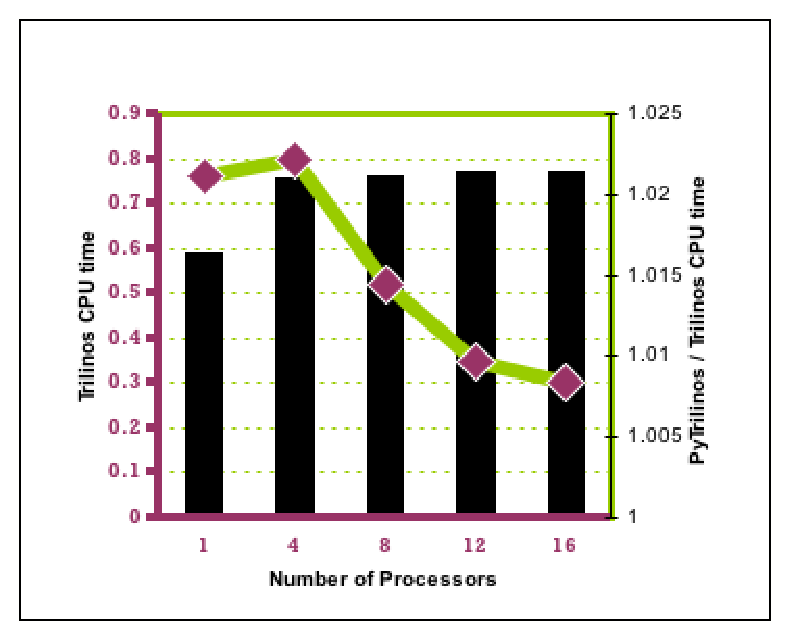
\includegraphics[width=7cm]{scalability-1k.eps}
\caption{Wall-clock time (in seconds) on 16-node Linux/GCC cluster for the
  codes reported in Table~\ref{tab:code_parallel_matvec}. The bars report the
time required by Trilinos, while the line reports the ratio between the time
required by PyTrilinos and the time required by Trilinos.}
\label{fig:time_parallel_matvec}
\end{center}
\end{figure}
%
%-----------------------------------------------------------------------------
\section{Performance Considerations}
\label{sec:performance}
%-----------------------------------------------------------------------------

The conclusion of the previous section is that fine-grained loops in
Python can be inefficient and should be avoided in the kernels of a
scientific code when speed is an issue.  Often, however, there is no
coarse-grained command available to do the same job efficiently.  One
example of this, that we will explore in this section, is solver
algorithms that use callbacks.

The NOX module implements nonlinear solvers at a relatively high
level, and expects the user to provide functions to compute residual
values, Jacobian matrices, and/or preconditioning matrices, depending
on the needs of the algorithm.  For example, when NOX needs a residual
computed, it calls a function set by the user to do the job.  When NOX
is accessed via PyTrilinos in Python, this callback function is by
necessity a Python function.  Unfortunately, it is a Python function
typically expected to perform fine-grained calculations, and so can be
an important source of inefficiencies.

Fortunately, there are ways to reduce these inefficiencies, and we
will explore two of them here.  Both methods substitute compiled loops
for Python loops, although by two different mechanisms.  The first is
using array slice syntax, and the second is using the {\tt weave}
module~\cite{Weave-Users-Guide}, a component of SciPy that can compile
and run embedded C or C++ code within a Python function.

We will demonstrate the advantages of these approaches by way of a
case study, involving the solution of a common nonlinear flow test
case, the incompressible lid-driven cavity problem~\cite{Ghia},
expressed here in terms of the stream function and vorticity.  The
stream function $\psi$ is defined implicitly in terms of the $x-$
and $y-$ flow velocity components $u$ and $v$:
\begin{equation}
  \label{eq:velocities}
  u = \frac{\partial \psi}{\partial x}, v = -\frac{\partial
    \psi}{\partial x}.
\end{equation}
The vorticity $\zeta$ is defined as the curl of the velocity.  In 2D,
this is always a vector perpendicular to the plane of the problem, and
so is treated as a scalar.  The relationship between stream function
and vorticity is therefore
\begin{equation}
  \label{eq:streamfunction}
  \left(\frac{\partial^2}{\partial x^2} + \frac{\partial^2}{\partial
    y^2}\right) \psi = -\zeta.
\end{equation}
The final governing equation can be obtained by taking the curl of the
incompressible momentum equation to obtain
\begin{equation}
  \label{eq:vorticity}
  \left[-\frac{\partial^2}{\partial x^2} - \frac{\partial^2}{\partial
    y^2} + Re \left(u \frac{\partial}{\partial x} + v
  \frac{\partial}{\partial y} \right)\right] \zeta = 0,
\end{equation}
where $Re$ is the Reynolds number.  The system is completed by
specifying the boundary conditions.  For the driven cavity problem,
the domain is the unit square with the no-slip condition applied to
all four walls.  That is, on the boundaries, we impose $u=v=0$ except
for the top boundary, which slides with a tangential velocity $u=1$.

The ``naive'' way to implement a Python function to compute, for
example, equations~\ref{eq:velocities}, using central differences on a
uniform grid of mesh size $h$, would be
\begin{verbatim}
    for i in xrange(1,nx-1):
       for j in xrange(1,ny-1):
          u[i,j] = (psi[i,j+1] - psi[i,j-1]) / (2*h)
          v[i,j] = (psi[i-1,j] - psi[i+1,j]) / (2*h)
\end{verbatim}
A second, and preferable, way to implement these equations would be to
use array slice syntax.  This forces the loops to be executed by the
underlying compiled Numeric code, and is more efficient:
\begin{verbatim}
    u[1:-1,1:-1] = (psi[2:,1:-1] - psi[0:-2,1:-1]) / (2*h)
    v[1:-1,1:-1] = (psi[1:-1,0:-2] - psi[1:-1,2:]) / (2*h)
\end{verbatim}
This approach is not always possible, especially if the governing
equation to be approximated is particularly complex.  A third way to
increase the efficiency of such a block of code would be to use the
{\tt weave} module:
\begin{verbatim}
    import weave
    code  = """
            for (int i=1; i<nx-1; ++i) {
              for (int j=1; j<ny-1; ++j) {
                u(i,j) = (psi(i,j+1) - psi(i,j-1)) / (2*h);
                v(i,j) = (psi(i-1,j) - psi(i+1,j)) / (2*h);
              }
            }
            """
    weave.inline(code,
                 ['u','v','psi','nx','ny','h'],
                 type_converters = weave.converters.blitz)
\end{verbatim}
It is not our purpose here to describe how the {\tt weave} module
works.  However, the meaning of the code should be clear: a Python
string is defined with valid C++ code and this string is passed to the
{\tt weave} module {\tt inline} function, along with the names of
variables that are to be passed to and from the embedded code, and an
optional specification for how those variables are to be converted.

\begin{table}
  \begin{center}
    \begin{tabular}{| r | c | l | r | l |}
      \hline
      \# & Equation                 & Method       & Solution Time & Notes \\
      \hline
      1 & All                       & naive        & 29.12 & Baseline \\
      2 & BCs                       & slice syntax & 26.05 & \\
      3 & BCs                       & weave        & 28.90 & Slice syntax is preferable \\
      4 & (\ref{eq:streamfunction}) & slice syntax & 19.99 & \\
      5 & (\ref{eq:streamfunction}) & weave        & 19.20 & Weave is slightly preferable \\
      6 & (\ref{eq:vorticity})      & weave        &  6.99 & Slice syntax complicated \\
      7 & (\ref{eq:velocities})     & slice syntax &  1.23 & \\
      8 & (\ref{eq:velocities})     & weave        &  1.44 & Slice syntax is preferable \\
      \hline
    \end{tabular}
    \caption{Case study of applying more efficient computational
      methods to Python callback functions for solving a $21\times21$
      Driven Cavity problem.}
    \label{tab:callbacks}
  \end{center}
\end{table}

Table~\ref{tab:callbacks} describes the process and results of
incrementally applying more efficient computational techniques to a
Python script that uses PyTrilinos.NOX to solve our driven cavity
problem on a $21\times21$ grid.  Line 1 is the baseline, in which all
the callback functions are written in the ``naive'' fine-grained
manner, taking just over 29 seconds to solve.  At line 2, we have
substituted array slice syntax for computing the boundary conditions,
shaving about 3 seconds off of our total solution time.  Line 3 is the
same for BCs computed using weave.  Note that in this instance, the
slice syntax is faster, and is the method we keep in the code.

Lines 4 and 5 refer to solving the stream function
equation~(\ref{eq:streamfunction}) with slice syntax and weave,
respectively.  In this case, weave is slightly faster, and that is the
version we keep, for an additional savings of about 7 seconds.  We
postulate that for ``small'' array sizes (1D boundaries in this case),
slice syntax is the most efficient approach, while for ``larger''
arrays (2D in this case), {\tt weave} will generally perform better.

For the vorticity equation~(\ref{eq:vorticity}) at line 6, we assume
this trend will hold and only implement the {\tt weave} method, which
saves an additional 12 seconds.  We note also that
equation~(\ref{eq:vorticity}) is more complicated than
equation~(\ref{eq:streamfunction}) and thus harder to implement with
array slice syntax.

The final two lines of the table, 7 and 8, describe the results for
converting the computational method for the velocities,
equation~(\ref{eq:velocities}).  Somewhat surprisingly, the array
slice syntax gives a slightly more efficient result even though this
is a ``larger'' 2D calculation rather than a 1D boundary computation.
This is most likely due to the simplicity of the formulas.  In the
end, we chose to keep the {\tt weave} version, because we could more
easily implement nonuniform mesh sizes.  Either way, the savings was
over 5.5 seconds, bringing the overall savings to just over 27.5
seconds and a speedup factor of over 20.

%
%-----------------------------------------------------------------------------
\section{Concluding Remarks}
\label{sec:concluding}
%-----------------------------------------------------------------------------

In this paper we have presented an overview of the \PyTrilinos\
project, an effort to facilitate the design, integration and ongoing
support of Python access to a large collection of mathematical
software libraries. \PyTrilinos\ provides a simple but powerful
rapid development environment, along with the integration tools
needed to apply it in realistic environments. In our opinion, the
most significant impact of \PyTrilinos\ is in the following areas:

\begin{itemize}

\item {\bf Rapid Prototyping.}  Because Python is a simple language,
  coding is much faster than in other languages. For example, its
  dynamic typing, built-in containers, and garbage collection
  eliminate much of the manual bookkeeping code typically required in
  languages like C or C++. As most bookkeeping code is missing, Python
  programs are easier to understand and more closely reflect the
  actual problem they're intended to address.  Often, well-written
  Python code looks like pseudo code, and as such it is easier to
  write, read, and maintain.

\item {\bf Brevity.} Python codes can be short and concise. Since
  things like type declaration, memory management, and common data
  structure implementations are absent, Python programs are typically
  a fraction of their C or C++ equivalents.  Brevity is also promoted
  by the object-oriented design of both \PyTrilinos\ and Trilinos
  itself.  Python scripts are short, generally with few jump
  statements, and therefore have good software metrics in terms of
  code coverage.

\item {\bf Modularity.} Python allows the code to be organized in
  reusable, self-contained modules.  This also reflects the natural
  structure of Trilinos itself. Since Python supports both structured
  and object-oriented design, users can adopt their preferred way of
  writing code.

\item {\bf Reusability.} Because Python is a high-level,
  object-oriented language, it encourages writing reusable software
  and well-designed systems.

%\item {\bf Legacy code migration.} Moving existing code from C/C++ to
  %Python makes it simpler and more flexible.  Modern numerical
  %algorithms are complex, and both the testing and fine tuning of
  %already developed algorithms, or the development of brand new ones
  %require a massive investment, for which rapid prototyping is
  %essential.
  %On the other hand, programmers simply cannot ignore
  %efficiency completely. Our approach is the following:
  %We use Python
  %when speed of development matters, compiled languages when
  %efficiency dominates, and combinations of the two when our goals are
  %not absolute.

\item {\bf Explorative Computation.} Since Python is an interpreted
  and interactive scripting language, the user can undertake
  computations in an explorative and dynamic manner. Intermediate
  results can be examined and taken into account before the next
  computational step, without the compile-link-run cycle typical of C
  or C++.

\item {\bf Integration.} Python was designed to be a ``glue'' language
  and \PyTrilinos\ relies on the ability to mix components written in
  other languages. C, C++ and FORTRAN code is called, but note that
  Python programmers don't need to care.  Python lends itself to
  experimental, interactive program development, and encourages
  developing systems incrementally by testing components in isolation
  and putting them together later.  By themselves, neither C nor
  Python is adequate to address typical development bottlenecks;
  together, they can do much more.  The model we are using splits the
  work effort into {\sl front-end} components that can benefit from
  Python's easy-of-use and {\sl back-end} modules that require the
  efficiency of compiled languages like C, C++, or FORTRAN.

\item {\bf Software Quality.} Software quality is of vital importance
  in the development of numerical libraries. If the quality of the
  software used to produce a new computation is questionable, then the
  result must be treated with caution as well. If, however, the
  quality of the software is high, it can reliably be made available
  to other research groups.

  Producing high quality software for state-of-the-art algorithms is a
  challenging goal, since research codes are often developed by
  several different programmers at the same time. Therefore, the
  production of high quality software requires a comprehensive set of
  testing programs. A way to do that without influencing the rapid
  development of prototype code, is to write tests in Python. By
  helping to detect defects, PyTrilinos can become an important
  testing tool for Trilinos itself. (Clearly, PyTrilinos tests require
  a bug-free interface between Trilinos and PyTrilinos.) Using
  PyTrilinos in the Trilinos test harness, one can experiment with the
  code to detect and manage dynamic errors, while static errors (like
  argument checking) must be detected by other types of testing.

\item {\bf Stability.} The only Python module on which PyTrilinos
  depends is Numeric, for both serial and parallel applications. Since
  Numeric is a well-supported and stable module, users can develop
  their applications based on PyTrilinos with no need to change or
  update them in a near future.

\item {\bf Data Input.} All scientific applications require data to be
  passed into the code.  Typically, this data is read from one or more
  files and often the input logic becomes extensive in order to make
  the code more flexible.  In other words, the scientific code
  developers often find themselves implementing a rudimentary
  scripting language to control their application.  We have found that
  applications developed in Python avoid this distraction from more
  scientific work because the Python scripts themselves become
  high-level ``input files,'' complete with variable definitions,
  looping capabilities and every other Python feature.

\end{itemize}

\smallskip

%With \PyTrilinos, it is no longer necessary to choose between fast development
%and fast execution.
Of course, Python (and by extension PyTrilinos) is not the perfect
language or environment for all problems. The most important problems
we have encountered are:

\begin{itemize}

\item {\bf Portability.} \PyTrilinos\ is developed concurrently on
  both Linux and Mac OS X, and it should port successfully to most
  other platforms where Trilinos, Python, Numeric and SWIG are
  available. However, configuring Trilinos, and thus \PyTrilinos, for
  a new platform can be a non-trivial exercise.

\item {\bf Shared Libraries on Massively Parallel Computers.} Another
  problem is related to the shared library approach, which is the
  easiest way of integrating third-party libraries in Python. Most
  massively parallel computers do not support shared libraries,
  therefore making Python scripts unusable for very large scale
  computations.

\item {\bf Lack of Compile-time Checks.} In Python all checks must be
  performed at run-time.  Furthermore, Python does not support strong
  typing of variables, so user mistakes related to incorrect variable
  usage can be a challenge to find and correct, where these types of
  mistakes would be caught quickly by a strongly-typed language and
  compiling system such as C++ and Java.

\item {\bf Performance Considerations.}  By using a Python wrapper, a
  performance penalty is introduced due to decoding of Python code,
  the execution of wrapped code, and returning the results in a
  Python-compliant format. These tasks may require thousands of CPU
  cycles, therefore it is important to recognize this situation when
  it occurs.  The performance penalty is small if the C/C++ function
  does a lot of work.  Therefore, for rarely called functions, this
  penalty is negligible.  All performance critical kernels should be
  written in C, C++, or Fortran, and everything else can be in Python,
  as we have shown for model problems in
  Sections~\ref{sec:comparison_python}, \ref{sec:comparison_matlab}
  and \ref{sec:comparison_trilinos}.

  This is especially critical in applications where function callbacks
  are used.  For example, in the NOX nonlinear solver module, it is
  common to set up an interface that specifies functions that NOX
  should call in order to compute the nonlinear equation to be solved
  or its Jacobian.  When such an interface is defined in Python, these
  functions are of necessity Python functions.  We have had success
  with SWIG, the {\tt weave} module and even Numeric array syntax.

  {\bf Last sentence is difficult to read}

\item {\bf Management of C/C++ Arrays.} Although SWIG makes it easy to
  wrap Python's lists as C and C++ arrays (and vice-versa), this
  process still requires the definition of wrappers in the interface
  file, that converts the array into a list, or a list into an
  array. Without an explicit wrapper, the proper handling of arrays
  can result in non-intuitive code, or memory leaks.

\item {\bf Limited Templated Code.} Most object-oriented numerical
  libraries are currently adopting massive template support, and
  templates have no meaning in Python.  This means that the interface
  writer has to select {\sl a-priori} which instances of the templated
  class will be included.  This is somewhat ironic, because pure
  Python code can be viewed as ``automatically'' templated, since
  rigorous type checking is not performed and expressions simply
  require that the specified operators and methods exist for any given
  object.  However, wrapped code must be type-checked ``under the
  covers.''

\end{itemize}

\smallskip

To summarize, the most important feature of Python is its powerful but
simple programming environment designed for development speed and for
situations where the complexity of compiled languages can be a
liability. Of course, Python enthusiasts will point out several other
strengths of the language; our aim is to show that Python can be
successfully used to develop and access state-of-the-art numerical
solver algorithms, in both serial and parallel environments.

We believe that \PyTrilinos\ is a unique effort, since for the first
time a large number of high-performance algorithms for distributed
sparse linear algebra has been made easily available from a scripting
language.  None of the previously reported projects for scientific
computing with Python handles sparse and distributed matrices, or the
diversity of solver algorithms. We hope that PyTrilinos can help to
make the development cycle of high-performance numerical algorithms
more efficient and productive.

\bigskip

{\bf Add other keywords?}

{\bf running title (in markboth()?}

%-----------------------------------------------------------------------------%
\bibliographystyle{acmtrans}
\bibliography{paper}
%-----------------------------------------------------------------------------%

\end{document}
